\documentclass{standalone}
\usepackage{tikz}
\usetikzlibrary{patterns}
\usetikzlibrary{positioning}
\usetikzlibrary{patterns, positioning}
\usetikzlibrary{shapes.misc}
\usepackage[outline]{contour}
\contourlength{1.5pt} 
\usepackage[sfdefault]{ClearSans}

\begin{document}
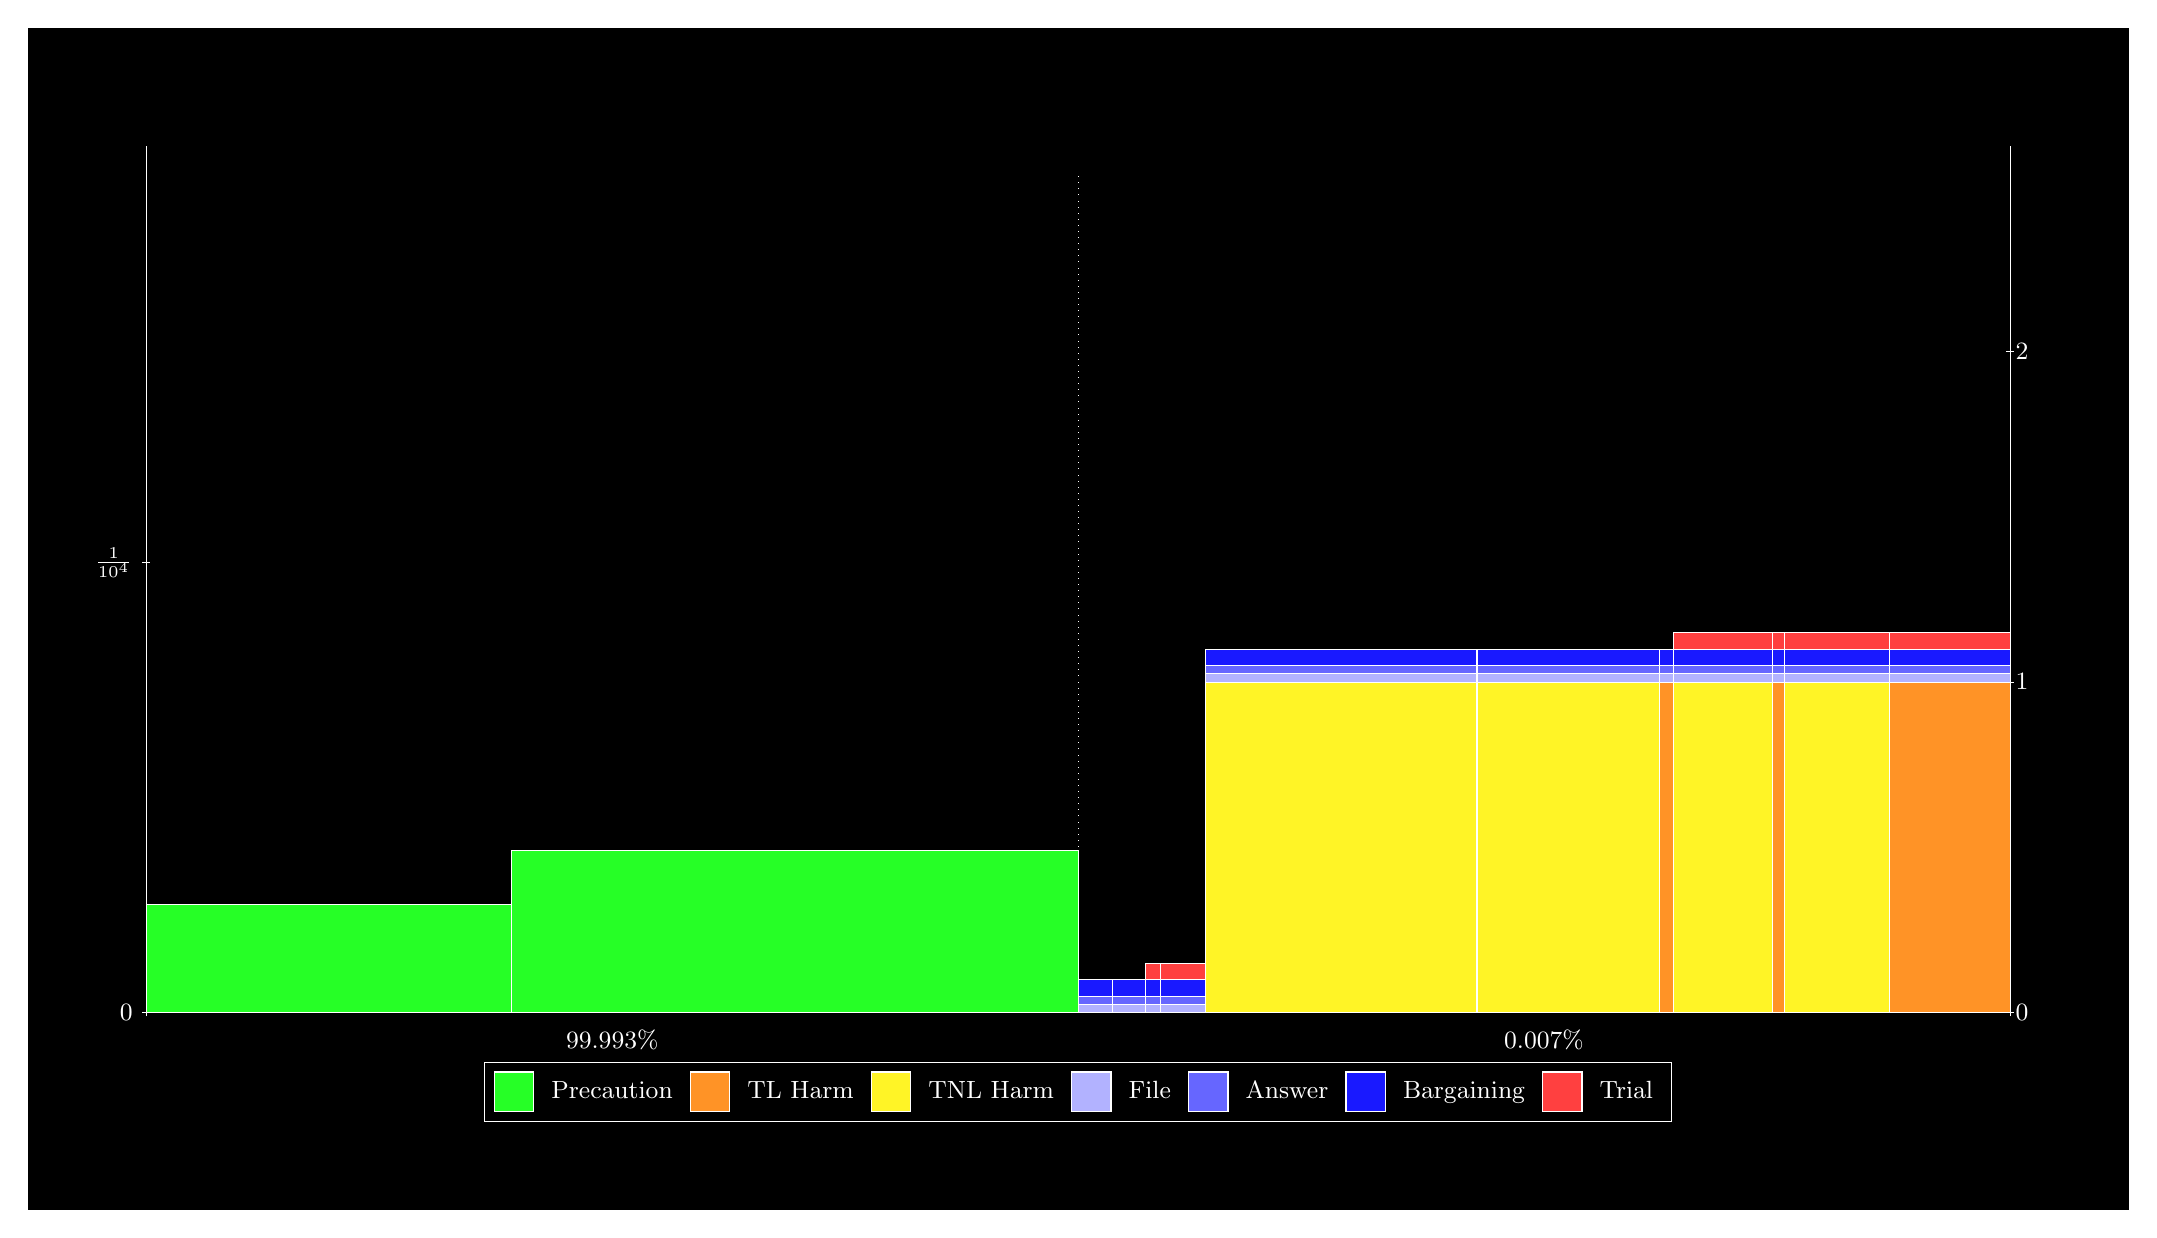
\begin{tikzpicture}
\draw[fill=black] (0,0) rectangle (26.667,15);
\draw[fill=green!85,draw=white,very thin] (1.5,2.5) rectangle (6.1372,3.8713);
\draw[fill=green!85,draw=white,very thin] (6.1372,2.5) rectangle (13.333,4.557);
\draw[fill=green!85,draw=white,very thin] (13.333,2.5) rectangle (13.772,2.5001);
\draw[fill=blue!30,draw=white,very thin] (13.333,2.5001) rectangle (13.772,2.6051);
\draw[fill=blue!60,draw=white,very thin] (13.333,2.6051) rectangle (13.772,2.71);
\draw[fill=blue!90,draw=white,very thin] (13.333,2.71) rectangle (13.772,2.9199);
\draw[fill=green!85,draw=white,very thin] (13.772,2.5) rectangle (14.187,2.5002);
\draw[fill=blue!30,draw=white,very thin] (13.772,2.5002) rectangle (14.187,2.6051);
\draw[fill=blue!60,draw=white,very thin] (13.772,2.6051) rectangle (14.187,2.7101);
\draw[fill=blue!90,draw=white,very thin] (13.772,2.7101) rectangle (14.187,2.92);
\draw[fill=green!85,draw=white,very thin] (14.187,2.5) rectangle (14.379,2.5001);
\draw[fill=blue!30,draw=white,very thin] (14.187,2.5001) rectangle (14.379,2.6051);
\draw[fill=blue!60,draw=white,very thin] (14.187,2.6051) rectangle (14.379,2.71);
\draw[fill=blue!90,draw=white,very thin] (14.187,2.71) rectangle (14.379,2.9199);
\draw[fill=red!75,draw=white,very thin] (14.187,2.9199) rectangle (14.379,3.1299);
\draw[fill=green!85,draw=white,very thin] (14.379,2.5) rectangle (14.944,2.5002);
\draw[fill=blue!30,draw=white,very thin] (14.379,2.5002) rectangle (14.944,2.6051);
\draw[fill=blue!60,draw=white,very thin] (14.379,2.6051) rectangle (14.944,2.7101);
\draw[fill=blue!90,draw=white,very thin] (14.379,2.7101) rectangle (14.944,2.92);
\draw[fill=red!75,draw=white,very thin] (14.379,2.92) rectangle (14.944,3.1299);
\draw[fill=green!85,draw=white,very thin] (14.944,2.5) rectangle (18.389,2.5001);
\draw[fill=yellow!85,draw=white,very thin] (14.944,2.5001) rectangle (18.389,6.6985);
\draw[fill=blue!30,draw=white,very thin] (14.944,6.6985) rectangle (18.389,6.8034);
\draw[fill=blue!60,draw=white,very thin] (14.944,6.8034) rectangle (18.389,6.9084);
\draw[fill=blue!90,draw=white,very thin] (14.944,6.9084) rectangle (18.389,7.1183);
\draw[fill=green!85,draw=white,very thin] (18.389,2.5) rectangle (18.397,2.5001);
\draw[fill=orange!85,draw=white,very thin] (18.389,2.5001) rectangle (18.397,6.6985);
\draw[fill=blue!30,draw=white,very thin] (18.389,6.6985) rectangle (18.397,6.8034);
\draw[fill=blue!60,draw=white,very thin] (18.389,6.8034) rectangle (18.397,6.9084);
\draw[fill=blue!90,draw=white,very thin] (18.389,6.9084) rectangle (18.397,7.1183);
\draw[fill=green!85,draw=white,very thin] (18.397,2.5) rectangle (20.718,2.5002);
\draw[fill=yellow!85,draw=white,very thin] (18.397,2.5002) rectangle (20.718,6.6985);
\draw[fill=blue!30,draw=white,very thin] (18.397,6.6985) rectangle (20.718,6.8035);
\draw[fill=blue!60,draw=white,very thin] (18.397,6.8035) rectangle (20.718,6.9085);
\draw[fill=blue!90,draw=white,very thin] (18.397,6.9085) rectangle (20.718,7.1184);
\draw[fill=green!85,draw=white,very thin] (20.718,2.5) rectangle (20.894,2.5002);
\draw[fill=orange!85,draw=white,very thin] (20.718,2.5002) rectangle (20.894,6.6985);
\draw[fill=blue!30,draw=white,very thin] (20.718,6.6985) rectangle (20.894,6.8035);
\draw[fill=blue!60,draw=white,very thin] (20.718,6.8035) rectangle (20.894,6.9085);
\draw[fill=blue!90,draw=white,very thin] (20.718,6.9085) rectangle (20.894,7.1184);
\draw[fill=green!85,draw=white,very thin] (20.894,2.5) rectangle (22.149,2.5001);
\draw[fill=yellow!85,draw=white,very thin] (20.894,2.5001) rectangle (22.149,6.6985);
\draw[fill=blue!30,draw=white,very thin] (20.894,6.6985) rectangle (22.149,6.8034);
\draw[fill=blue!60,draw=white,very thin] (20.894,6.8034) rectangle (22.149,6.9084);
\draw[fill=blue!90,draw=white,very thin] (20.894,6.9084) rectangle (22.149,7.1183);
\draw[fill=red!75,draw=white,very thin] (20.894,7.1183) rectangle (22.149,7.3282);
\draw[fill=green!85,draw=white,very thin] (22.149,2.5) rectangle (22.302,2.5001);
\draw[fill=orange!85,draw=white,very thin] (22.149,2.5001) rectangle (22.302,6.6985);
\draw[fill=blue!30,draw=white,very thin] (22.149,6.6985) rectangle (22.302,6.8034);
\draw[fill=blue!60,draw=white,very thin] (22.149,6.8034) rectangle (22.302,6.9084);
\draw[fill=blue!90,draw=white,very thin] (22.149,6.9084) rectangle (22.302,7.1183);
\draw[fill=red!75,draw=white,very thin] (22.149,7.1183) rectangle (22.302,7.3282);
\draw[fill=green!85,draw=white,very thin] (22.302,2.5) rectangle (23.632,2.5002);
\draw[fill=yellow!85,draw=white,very thin] (22.302,2.5002) rectangle (23.632,6.6985);
\draw[fill=blue!30,draw=white,very thin] (22.302,6.6985) rectangle (23.632,6.8035);
\draw[fill=blue!60,draw=white,very thin] (22.302,6.8035) rectangle (23.632,6.9085);
\draw[fill=blue!90,draw=white,very thin] (22.302,6.9085) rectangle (23.632,7.1184);
\draw[fill=red!75,draw=white,very thin] (22.302,7.1184) rectangle (23.632,7.3283);
\draw[fill=green!85,draw=white,very thin] (23.632,2.5) rectangle (25.167,2.5002);
\draw[fill=orange!85,draw=white,very thin] (23.632,2.5002) rectangle (25.167,6.6985);
\draw[fill=blue!30,draw=white,very thin] (23.632,6.6985) rectangle (25.167,6.8035);
\draw[fill=blue!60,draw=white,very thin] (23.632,6.8035) rectangle (25.167,6.9085);
\draw[fill=blue!90,draw=white,very thin] (23.632,6.9085) rectangle (25.167,7.1184);
\draw[fill=red!75,draw=white,very thin] (23.632,7.1184) rectangle (25.167,7.3283);
\draw[white,very thin] (1.5,2.5) -- (1.5,13.5);
\draw[white,very thin] (1.45,2.5) -- (1.55,2.5);
\node[font=\small,text=white, anchor=east] at (1.45, 2.5) {0};
\draw[white,very thin] (1.45,8.2139) -- (1.55,8.2139);
\node[font=\small,text=white, anchor=east] at (1.45, 8.2139) {$\frac{1}{10^{4}}$};

\draw[white,dotted,very thin] (13.333,2.83) -- (13.333,13.17);
\draw[white,very thin] (25.167,2.5) -- (25.167,13.5);
\draw[white,very thin] (25.117,2.5) -- (25.217,2.5);
\node[font=\small,text=white, anchor=west] at (25.117, 2.5) {0};
\draw[white,very thin] (25.117,6.6984) -- (25.217,6.6984);
\node[font=\small,text=white, anchor=west] at (25.117, 6.6984) {1};
\draw[white,very thin] (25.117,10.897) -- (25.217,10.897);
\node[font=\small,text=white, anchor=west] at (25.117, 10.897) {2};

\draw[white,very thin] (1.5,2.5) -- (25.167,2.5);
\draw[white,very thin] (1.5,2.45) -- (1.5,2.55);
\node[font=\small,text=white, anchor=north] at (1.5, 2.45) {};
\draw[white,very thin] (25.167,2.45) -- (25.167,2.55);
\node[font=\small,text=white, anchor=north] at (25.167, 2.45) {};

\node[font=\small,text=white,anchor=south] at (7.4167, 1.9) {99.993\%};
\node[font=\small,text=white,anchor=south] at (19.25, 1.9) {0.007\%};
\draw (13.3333,2.5) node (B) {};
\begin{scope}[align=center]
\matrix[scale=0.5,draw=white,below=0.5cm of B,nodes={draw},column sep=0.1cm]{
\node[rectangle,draw,minimum width=0.5cm,minimum height=0.5cm,fill=green!85]{}; & \node[draw=none,font=\small,text=white]{Precaution}; &
\node[rectangle,draw,minimum width=0.5cm,minimum height=0.5cm,fill=orange!85]{}; & \node[draw=none,font=\small,text=white]{TL Harm}; &
\node[rectangle,draw,minimum width=0.5cm,minimum height=0.5cm,fill=yellow!85]{}; & \node[draw=none,font=\small,text=white]{TNL Harm}; &
\node[rectangle,draw,minimum width=0.5cm,minimum height=0.5cm,fill=blue!30]{}; & \node[draw=none,font=\small,text=white]{File}; &
\node[rectangle,draw,minimum width=0.5cm,minimum height=0.5cm,fill=blue!60]{}; & \node[draw=none,font=\small,text=white]{Answer}; &
\node[rectangle,draw,minimum width=0.5cm,minimum height=0.5cm,fill=blue!90]{}; & \node[draw=none,font=\small,text=white]{Bargaining}; &
\node[rectangle,draw,minimum width=0.5cm,minimum height=0.5cm,fill=red!75]{}; & \node[draw=none,font=\small,text=white]{Trial}; \\\\
};\end{scope}

\end{tikzpicture}
\end{document}